\documentclass[final,5p,times,twocolumn]{elsarticle}
\usepackage{caption}
\usepackage{amssymb}
\usepackage{amsmath}
\usepackage{multirow}
\usepackage{booktabs}
\usepackage{stfloats}
\usepackage{threeparttable}
\usepackage{graphicx}
\usepackage{array}
\usepackage{pifont}
\usepackage{tabularx}
\usepackage{longtable}
\usepackage[hyphens]{url}
\usepackage[colorlinks,breaklinks]{hyperref}
\usepackage{tikz}
\usepackage{placeins}
\newcommand{\cmark}{\ding{51}}
\usetikzlibrary{shapes, arrows.meta, positioning, fit, calc}
\usepackage{rotating}

\begin{document}
\begin{frontmatter}

\title{DentalClaw: A Modular Workflow Platform for Standardized and Auditable Dental Imaging AI Experiments}

\begin{abstract}
\textit{Objectives:} Dental imaging artificial intelligence (AI) research depends on coordinated steps including data curation, preprocessing, model configuration, evaluation, and structured reporting, yet these tasks are often fragmented across scripts and manual procedures, making dental AI studies difficult to reproduce and review. This study evaluated DentalClaw, a natural-language-driven workflow platform that converts user intent into executable and auditable dental imaging AI pipelines.\\
\textit{Methods:} DentalClaw was implemented as a modular platform integrating intent parsing, method selection, dataset auditing, model execution, evaluation, and report generation. The system was assessed on representative 2D panoramic radiograph segmentation and 3D cone-beam computed tomography (CBCT) segmentation tasks, and its decision layer was evaluated across 30 prespecified natural-language intents spanning standard executable requests, ambiguous requests, trap (out-of-scope or quality-control-first) queries, and boundary cases.\\
\textit{Results:} DentalClaw completed end-to-end workflows for both representative public dental imaging tasks and generated standardized outputs including split files, prediction results, evaluation tables, and review-oriented reports. Compared with manually assembled script-based workflows, the platform reduced manual coordination time during dataset preparation and result organization while preserving a consistent execution trace. The intent-to-workflow decision evaluation achieved a study-defined weighted decision score of 0.958 (all 30 intents above the 0.70 pass threshold), higher than three general-purpose assistants (0.889--0.893) on the same requests and rubric, and no incorrect workflow was silently executed.\\
\textit{Conclusions:} DentalClaw demonstrated the feasibility of translating natural-language research intent into auditable and executable dental imaging AI workflows under representative settings. The study supports the platform as a workflow orchestration and validation framework rather than as a new segmentation model or as a standalone clinical decision-support system.\\
\textit{Clinical Significance:} By standardizing workflow execution and traceability, DentalClaw is designed to reduce the coordination burden of multi-step dental AI experiments while preserving a reviewable record of the data, configuration, and outputs associated with dental AI studies.
\end{abstract}

\begin{keyword}
Dental informatics \sep Artificial intelligence \sep Digital dentistry \sep Workflow automation \sep Auditable experiments \sep Cone-beam computed tomography \sep Panoramic radiography
\end{keyword}

\end{frontmatter}

\section{Introduction}

\begin{figure*}[t]
\centering
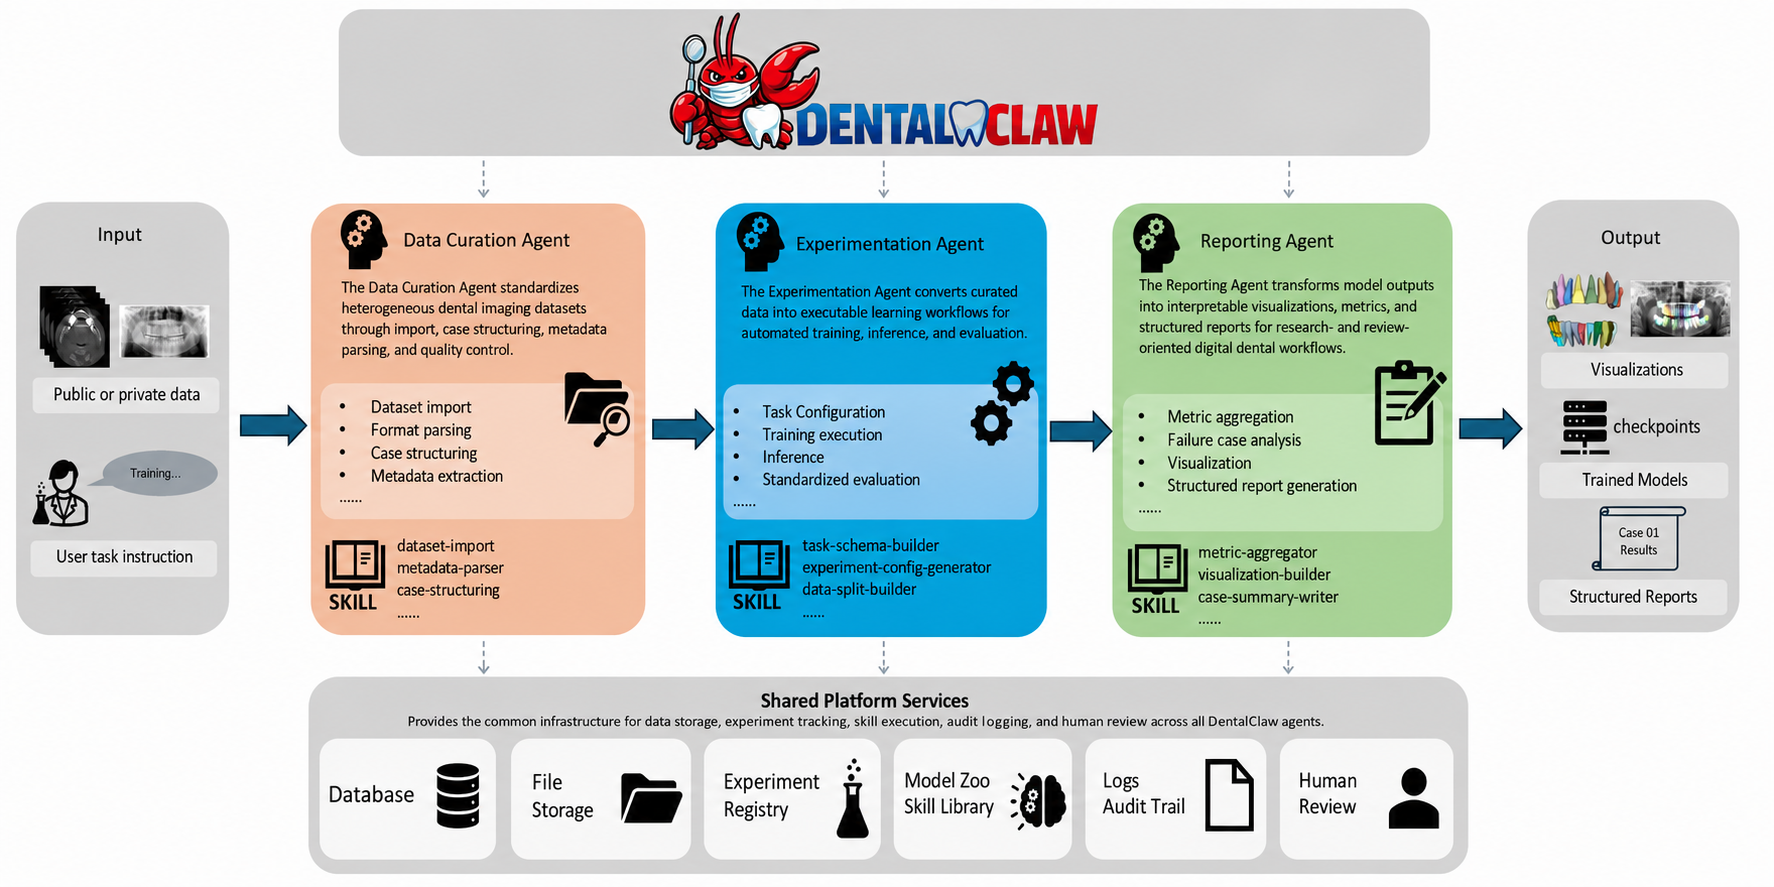
\includegraphics[width=0.72\textwidth]{Multi-agent system architecture of DentalClaw.png}
\caption{Overview of the DentalClaw architecture. Heterogeneous dental imaging inputs and researcher instructions are processed by a central coordinator and routed to specialized data-curation, experimentation, and reporting agents. Shared platform services provide dataset organization, model and skill libraries, audit logs, and human review support; the reporting agent transforms model outputs into research- and review-oriented structured reports.}
\label{fig:system_overview}
\end{figure*}

Dental imaging AI has become increasingly relevant for tooth segmentation, lesion detection, treatment planning support, and image-based diagnosis in digital dentistry~\cite{Horner2012,Kapila2015,Schwendicke2020,Shujaat2021}. In recent years, deep learning methods have shown strong performance in dental radiographs and CBCT analysis; however, the practical challenge of translating a study idea into a reproducible workflow remains substantial. In many real-world projects, the bottleneck is not the absence of a capable model but the fragmented process of dataset curation, annotation harmonization, preprocessing, model selection, evaluation, and final report generation~\cite{Schwendicke2021Checklist,Polizzi2023,Dot2024DentalSegmentator}. These steps are often implemented as ad hoc scripts or local procedures, which makes results difficult to reproduce, compare, and audit across studies.

This problem is amplified by the heterogeneity of dental imaging data: panoramic radiographs, periapical images, CBCT volumes, and clinical annotations differ in format, dimensionality, metadata structure, and quality-control requirements, and variations in labeling conventions, field-of-view completeness, and patient-level splitting can undermine reproducibility across institutions~\cite{Nemtoi2013,Schwendicke2021Checklist,Polizzi2023}. These issues are particularly relevant for clinicians and dental researchers who understand the clinical objective but lack the engineering infrastructure to execute the full workflow reliably.

Existing software tools partly address this challenge. General medical imaging frameworks such as nnU-Net~\cite{Isensee2021nnUNet}, MONAI~\cite{Cardoso2022MONAI}, and 3D Slicer~\cite{Fedorov2012Slicer} provide strong model-development primitives, while dental-specific tools often target a narrow task or a single modality. DentalClaw addresses a complementary need: it orchestrates the experimental workflow around user intent, converts natural-language requests into candidate executable routes, and records actions in an auditable form. In this sense, the platform is best understood as an orchestration layer rather than as a new segmentation model.

The platform incorporates six functional components: natural-language intent parsing; matching against an offline registry of validated, task-specific methods, independent of live search; automated dataset auditing and quality-control checks with deterministic case-level splitting; execution of registered methods only, including TTA and multi-model ensemble routes; prespecified evaluation metrics and standardized review-oriented reports that form an audit trail with plan files and execution logs; and a conservative fail-safe policy in which unsupported requests are rejected or clarified and agent-proposed external solutions require explicit human approval.

The objective of this study was to assess whether a researcher-oriented workflow platform could reduce the coordination burden of multi-step dental imaging AI research by transforming natural-language instructions into executable, reviewable, and traceable research pipelines. We evaluated DentalClaw on representative 2D panoramic radiograph segmentation and 3D CBCT segmentation tasks, and we assessed its decision pipeline on 30 prespecified intents spanning standard executable requests, ambiguous requests, trap (out-of-scope or quality-control-first) queries, and boundary cases. This design allows the platform to be judged not only by final segmentation metrics, but also by whether it can correctly map a user request to an appropriate workflow, maintain traceability, and prevent unsupported actions from being silently executed.

\begin{figure*}[b!]
\centering
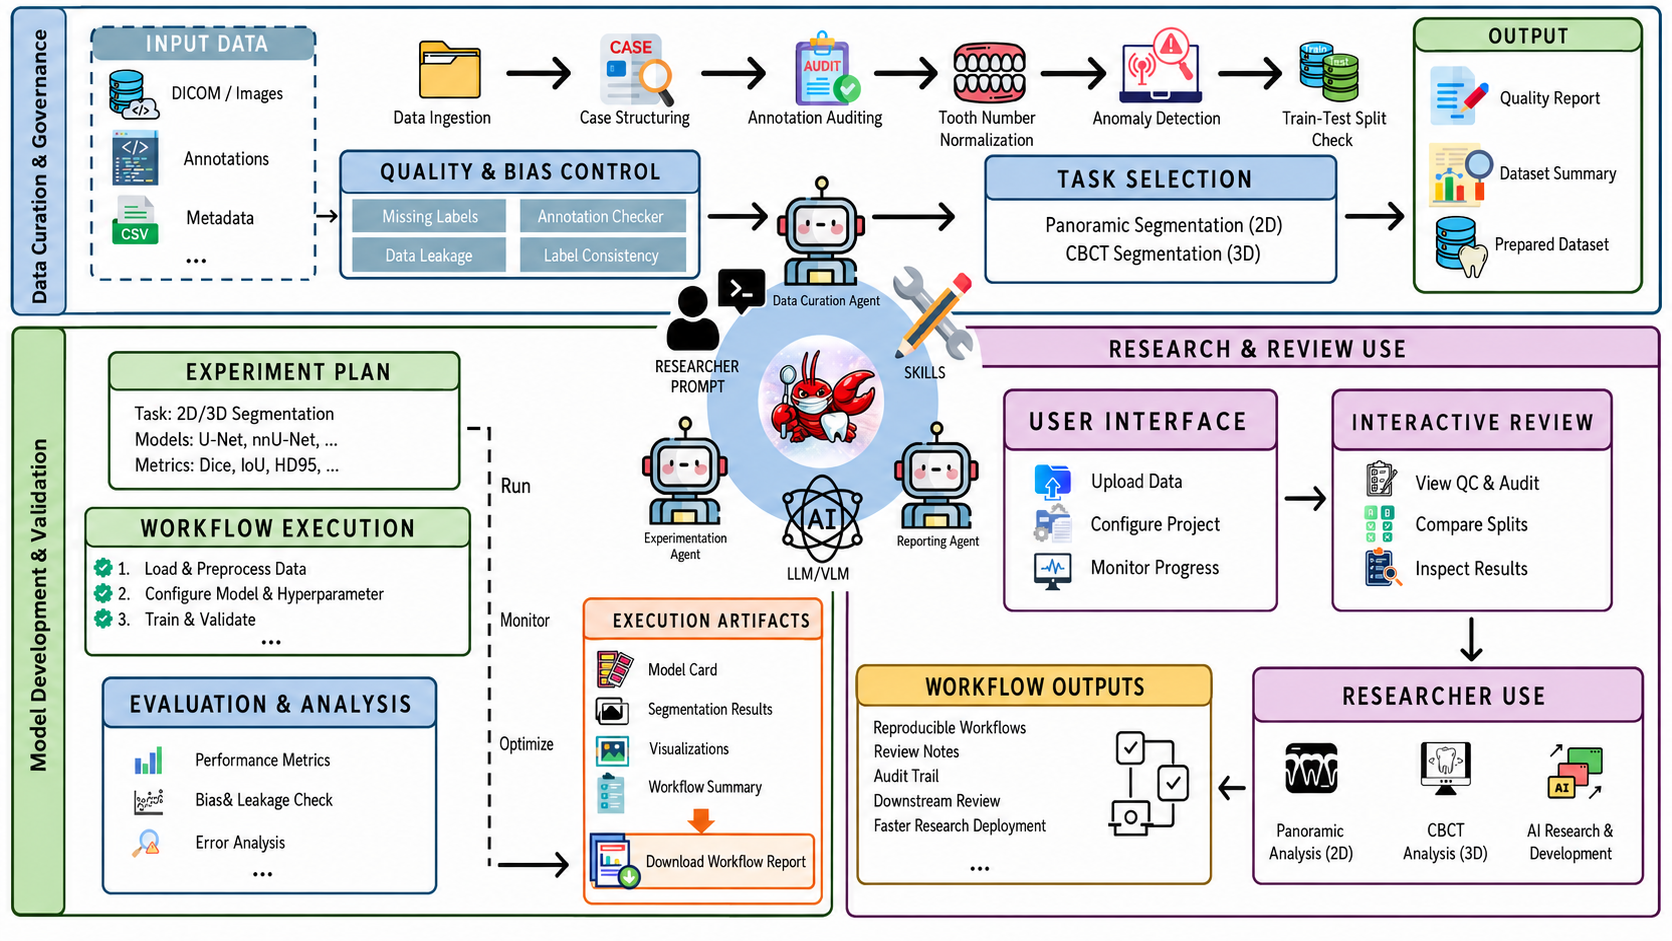
\includegraphics[width=0.72\textwidth]{Overall workflow of DentalClaw.png}
\caption{Overall workflow of DentalClaw. A researcher prompt is parsed into structured fields, matched against a registry of validated methods, and routed to either an executable path or a human-reviewed external proposal. Deterministic modules perform dataset preparation, model execution, evaluation, and reporting, producing execution artifacts, review notes, and an audit trail for downstream review.}
\label{fig:framework}
\end{figure*}

\section{Materials and methods}

\subsection{Study design and platform overview}
DentalClaw was implemented as a modular workflow platform built around OpenClaw~\cite{openclaw}. The system includes a natural-language reasoning layer, an offline method registry, dataset and quality-control modules, task-specific execution routes, and structured reporting. The agent parses a user request into structured fields including dataset, task family, modality, mode, and optional TTA or ensemble flags. It then performs registry lookup and, when necessary, proposal generation. In addition to single-model routes, the registry included a dedicated test-time augmentation (TTA) and multi-model ensemble inference route; TTA and ensemble flags parsed from natural-language requests were mapped to this route during method selection. The design is intentionally conservative: unsupported or ambiguous requests are rejected, while external proposals are surfaced for human review instead of being executed automatically.

The execution layer contains deterministic modules for dataset preparation, preprocessing, model training or inference, evaluation, and report generation, each storing its configuration, intermediate outputs, and workflow status for traceability. The reasoning agent constitutes the platform's decision layer: it decides which workflow should be attempted, while the deterministic execution layer runs only the validated route or an approved external proposal.

For the present study, the platform ran on a server with an NVIDIA GeForce RTX 3090 GPU. The decision layer used the OpenClaw runtime with DeepSeek V4 Pro as the primary reasoning backend (sampling temperature 0.1), constrained to return a structured JSON decision with a parsing fallback for malformed responses. Prompts contained only textual task descriptors, registry metadata, and codebase asset descriptions; raw images, annotations, and patient identifiers were processed locally and were never transmitted to the model API. Literature search over Europe PMC and arXiv served as auxiliary context for proposal generation and citation, whereas registry-based route selection remained deterministic and independent of live search results.

Because the reasoning agent is an external and potentially untrusted component, the platform treats its output as input to be validated rather than as code to be executed. The agent operates in a decision-only mode; all execution is delegated to local, versioned modules, and if the agent is unavailable or its decision cannot be parsed, the platform falls back to deterministic registry lookup and rejects the request when no validated method matches. Retrieved literature is used only as auxiliary context, never as executable instruction. External proposals remain non-executable until a user explicitly confirms them with the \texttt{--allow-external} flag, after which any externally sourced code is reviewed before it is adapted into the platform. API credentials are read from environment variables and are not embedded in prompts or stored in workflow logs; execution logs and agent traces are kept in per-run directories to support auditing. Residual risks, including prompt-injection attacks mediated by retrieved content or malicious file metadata, supply-chain risks of externally sourced code, and the absence of an independent security evaluation, are acknowledged in the Discussion.

\subsection{Agent decision pipeline}
The agent decision pipeline operated in five stages: (1) the natural-language request was parsed into structured fields (dataset, task family, modality, mode, and optional TTA or ensemble flags); (2) a task-aware literature search query was generated and run against Europe PMC and arXiv; (3) the offline method registry was queried for a validated executable path; (4) the agent synthesized the parsed intent, registry status, search results, and available codebase assets into one of three outcomes---\texttt{use\_registry}, \texttt{external\_proposal}, or \texttt{reject}; and (5) the final plan was serialized in a machine-readable file recording the selected method, decision rationale, cited references, prerequisite checks, and human-review requirement. This design distinguishes supported workflows, promising external options, and unsupported requests without silent fallback behavior, and creates a per-run record that supports reproducibility and downstream auditing of the exact intent, chosen route, and execution parameters.

\subsection{Datasets and representative workflows}
Two public datasets and one private dataset were used for validation. The Tufts Dental Database (TDD)~\cite{panetta2022tufts} was used for 2D panoramic radiograph segmentation. After automated audit and curation, 968 of 1051 cases were retained; excluded cases were dominated by missing masks and image--label mismatches. ToothFairy3~\cite{ToothFairyDataset1,ToothFairyDataset2,ToothFairyDataset3} was used for 3D CBCT segmentation, with 43 of 63 volumes passing eligibility checks; exclusions were dominated by metal artifacts and field-of-view anomalies. Ground-truth annotations for both public datasets were taken from the original dataset releases and were not re-annotated in this study.

A private panoramic dataset was also used for exploratory task extension and quality review. It included 290 images collected during routine clinical care between 2012 and 2024 under institutional ethical approval (PKUSSIRB-2025,107,012). Ground-truth annotations were provided by clinical experts as bounding boxes for pulp, root canal fillings, fillings, and periapical lesions; images with poor quality or incomplete dentition were excluded. While not the primary focus of the platform validation, this dataset tested how the system handled private, clinically relevant data and generated review-oriented outputs around real-world case quality.

\subsection{Workflow execution and quality control}
All datasets were converted to a canonical case-level representation (image references, annotation files, modality information, and workflow status) before model execution. Built-in quality-control functions then checked image completeness, annotation integrity, metadata consistency, and train--test leakage risk; the leakage checks included duplicate-identifier verification across splits, and no duplicate identifiers were found in any split. Train/validation/test splits were generated deterministically at the case level with a fixed random seed (42). For flagged cases, the platform recorded the issue category and handling decision, including normalization, exclusion, or manual review.

After validation, DentalClaw generated a task-specific execution plan specifying preprocessing rules, split assignment, output directories, and evaluation settings. For the 2D panoramic task, the platform configured nnU-Net v2 in its 2D full-resolution configuration for binary tooth segmentation (one class), with mean Dice as the primary evaluation metric and case-level splits of 900 training and 100 test cases. For the 3D CBCT task, the platform configured nnU-Net 3D full-resolution training together with U-Mamba and SwinUNETR model variants, test-time augmentation, and a multi-model ensemble route with post-processing; teeth (classes 1--32) and restorations (classes 33--35) were evaluated separately. The execution pipeline then invoked the selected model route, generated predictions, computed the prespecified metrics, and exported structured reports for downstream review. The complete training configuration, including optimizer, learning-rate schedule, augmentation, ensemble rules, and software versions, is provided in the Supplementary Methods.

\subsection{Evaluation protocol}
The evaluation strategy combined workflow-level validation (successful end-to-end completion, from dataset preparation to structured reporting) with intent-level decision testing. At the decision level, we constructed a six-dimension weighted evaluation framework across 30 prespecified intents covering four behavior classes: standard executable requests (5), boundary requests without a validated route (13), ambiguous requests (7), and trap (out-of-scope or quality-control-first) queries (5). The intent set spanned three dataset groups (TDD, ToothFairy3, private 2D) and four task families (2D segmentation, 3D segmentation, detection, classification), and included several requests whose task family was deliberately not stated in the request text. For each intent, the expected platform outcome (supported, executable, and target method) was predefined by the study team before evaluation, on the basis of the offline registry contents and the platform's documented scope. A decision was considered correct only when the selected route matched the intended dataset, task family, modality, and execution mode, or when the request was correctly rejected.

Each intent received a score computed as a weighted combination of six prespecified dimensions: planning (0.35), QC blocking (0.20), intent parsing (0.15), external proposal quality (0.15), ambiguity handling (0.10), and boundary identification (0.05). The weights were specified a priori by the study team to place the greatest emphasis on correct method selection and on correct accept/reject decisions, which are the behaviors most relevant to safe workflow execution. The overall score was then computed as the average of the per-intent scores, with intents scoring at or above 0.70 considered passing. The protocol follows recent practice in native-runtime agent evaluation, in which deterministic rule-based checks against prespecified expectations are preferred over task-oracle success alone~\cite{Ding2026WildClawBench}, and is further motivated by evidence that task success can conceal process-level anomalies in agent execution trajectories~\cite{Liu2026OpenClawBench}.

To contextualize the platform's decision behavior, the same 30 requests were issued to three general-purpose assistants---Copilot (GPT-5.6 Luna), Qwen (Qwen3.8-Max), and Claude Code with a DeepSeek V4 Pro backend, the same backend model used by the platform's reasoning layer---each in a fresh single-turn conversation with an identical preamble describing the datasets, registry, decision rules, and required JSON output format, without executing any code; the full comparison protocol is provided in the Supplementary Methods. Responses were scored with the same rubric against the same prespecified expectations. The rubric therefore measures decision fidelity, that is, agreement between platform behavior and the prespecified expected outcome of each request. Methodological appropriateness---which task family, evaluation unit, and metrics apply to each validated route---is encoded a priori in the registry specifications authored by the study team: each validated entry explicitly declares its required annotation type, evaluation unit, evaluation metrics, quality-control gates, and contraindications. Independent expert validation of these specifications against a formal rubric was not performed (see Discussion). For quality-control-first trap requests whose task family is not stated in the request text, the prespecified correct decision-level outcome is conservative clarification or rejection; execution-level quality-control blocking lies outside this decision-level protocol.

\section{Results}

\subsection{Workflow completion and execution traceability}
\begin{figure*}[!t]
\centering
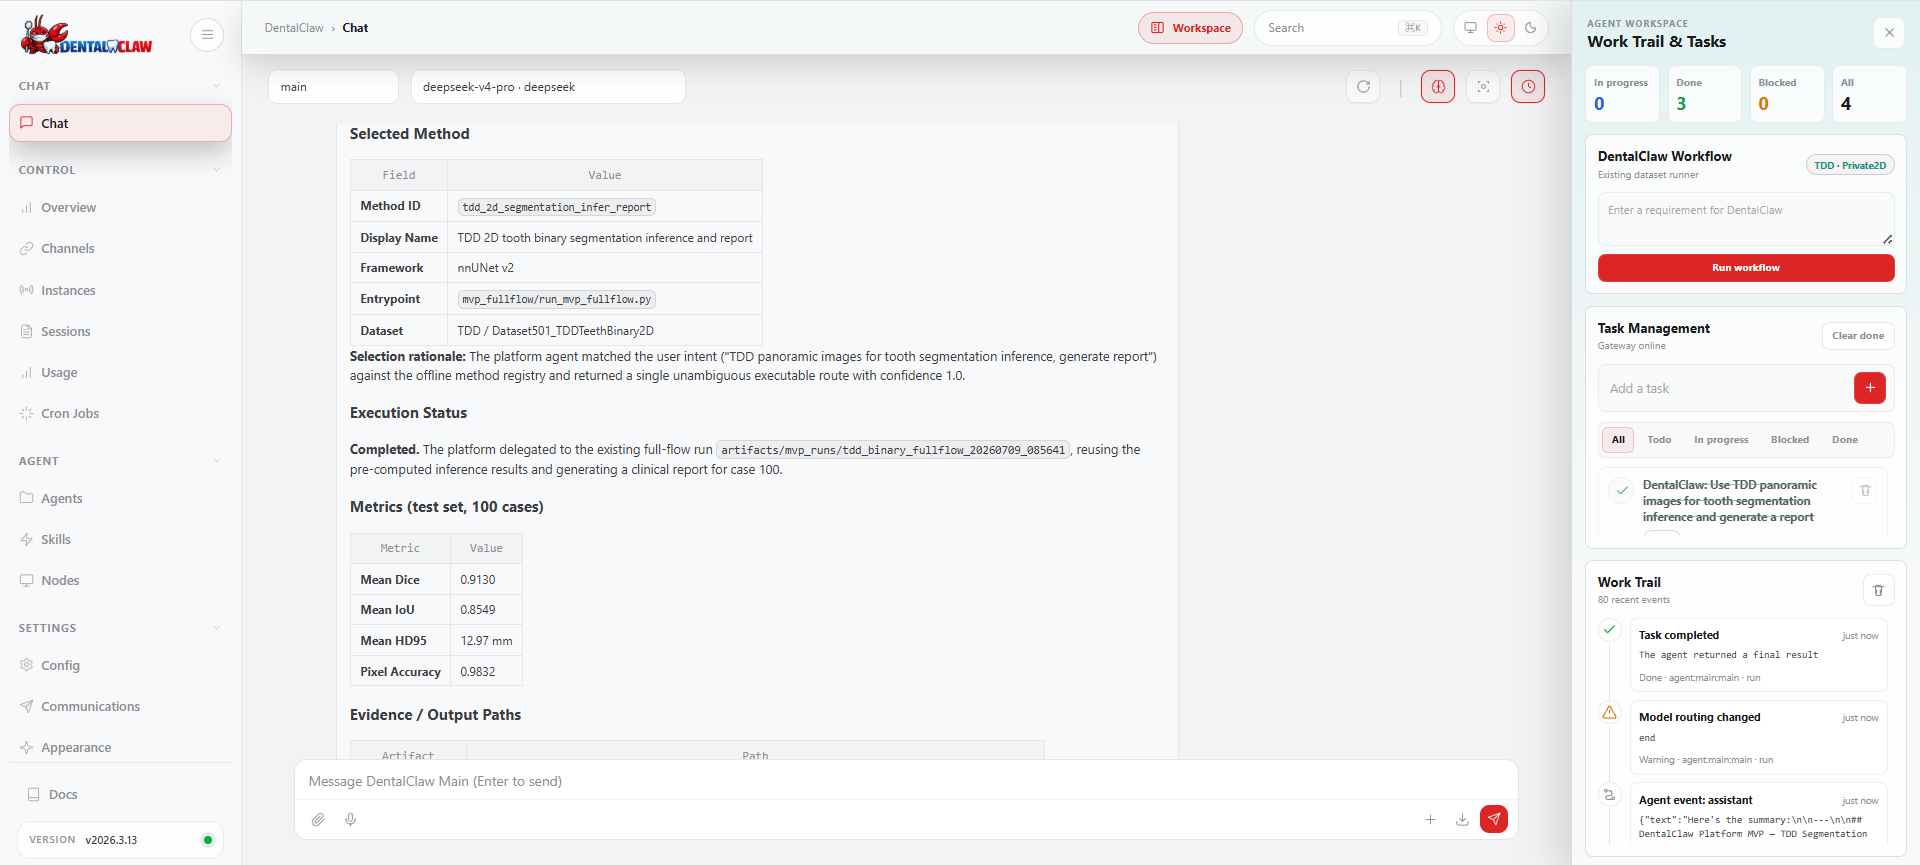
\includegraphics[width=0.65\textwidth]{Complete training.png}
\caption{Front-end workflow trace of DentalClaw showing the agent planning, task scheduling, and report-generation state during a completed run. The interface makes the decision and execution path visible for review and auditability.}
\label{fig:complete_training}
\end{figure*}

DentalClaw completed end-to-end workflows for both public datasets: in the 2D panoramic setting it executed dataset curation, model training, inference, evaluation, and structured reporting; in the 3D CBCT setting it handled volumetric data with modality-specific preprocessing, multi-model execution, and result aggregation under the same orchestration framework. Both workflows generated standardized outputs including manifests, split files, predictions, metrics tables, and review-oriented reports.

Beyond workflow completion, two configuration case studies exercised the platform's reusable-skill layer under the same audit and logging framework. On a TDD-derived 32-class panoramic tooth segmentation task, the platform orchestrated a trajectory of predefined configuration skills (intensity augmentation, cosine-annealed learning-rate schedule, AdamW optimizer, and test-time augmentation), improving the mean Dice score from 0.6163 to 0.6937 (HD95 from 83.15 to 38.54 mm); a documented comparison with configurations selected by three operators with differing AI backgrounds (a novice, a master's-level researcher, and an AI practitioner) is reported in the Supplementary Methods. On the 35-class CBCT task, platform-managed fusion of nnU-Net, SwinUNETR, and U-Mamba models with test-time augmentation and post-processing achieved mean Dice scores of 0.8058 for teeth and 0.7653 for restorations, from nnU-Net single-model baselines of 0.7038 and 0.6588. These outcomes indicate that the executed workflows produced reviewable performance results rather than silently failing; the complete trajectory tables are provided in the Supplementary Methods.

Workflow-level outcomes, including a manually assembled script workflow executed for comparison, are summarized in Supplementary Table~\ref{tab:supp_workflow}; the comparison is reported as a workflow demonstration rather than a controlled human-factor experiment. In the documented runs, the platform required substantially less operator coordination for dataset preparation and result organization, whereas model training time remained essentially unchanged, consistent with its role as a coordination layer rather than a training accelerator. An exploratory workflow on the private panoramic dataset further exercised the same intent-to-route and quality-review logic on clinically sourced images, supporting extensibility to private data.

\subsection{Intent-to-workflow decision evaluation}
To assess the agent's decision capability, we evaluated the full pipeline across 30 prespecified natural-language requests (Table~\ref{tab:assistant_comparison}). All five standard requests were routed to the correct registry method, and all 25 remaining requests---boundary, ambiguous, and trap---were blocked without execution (11 non-executable external proposals and 2 rejections for boundary requests, 4 clarifications and 3 proposals for ambiguous requests, and 2 clarifications and 3 proposals for trap requests). In no case was an unvalidated workflow silently executed.

\begin{table*}[!t]
\centering
\footnotesize
\caption{Decision-evaluation scores of DentalClaw and three general-purpose assistants on the same 30 prespecified requests under the same six-dimension rubric. Per-request scores, selected methods, and the full request texts are provided in Supplementary Table~\ref{tab:supp_intents}.}
\label{tab:assistant_comparison}
\begin{tabular}{l c c c c c c c}
\toprule
System & $n$ & Overall & Standard & Boundary & Ambiguous & Trap & Passed \\
\midrule
DentalClaw (platform) & 30 & \textbf{0.958} & 1.000 & 0.978 & \textbf{0.943} & 0.886 & 30/30 \\
Copilot (GPT-5.6 Luna) & 30 & 0.893 & 1.000 & 0.958 & 0.739 & 0.833 & 28/30 \\
Qwen (Qwen3.8-Max) & 30 & 0.891 & 1.000 & 0.958 & 0.739 & 0.818 & 28/30 \\
Claude Code (DeepSeek V4 Pro backend) & 30 & 0.889 & 1.000 & 0.954 & 0.739 & 0.818 & 28/30 \\
\bottomrule
\end{tabular}
\end{table*}

Two behavioral patterns emerged among the imperfect cases. For three trap queries and three ambiguous requests, the agent generated a non-executable external proposal instead of the stricter rejection or clarification behavior prespecified for those classes---prevented from automatic execution, since no proposal is executed without explicit approval, but indicating that proposal generation can occasionally override the more conservative specified behavior. Second, two classification requests were rejected outright, consistent with the registry scope policy. In every case the platform kept unvalidated proposals behind explicit human review.

Under the same rubric, the three assistants scored 0.893 (Copilot), 0.891 (Qwen), and 0.889 (Claude Code with a DeepSeek V4 Pro backend), all below the platform's 0.958 (Table~\ref{tab:assistant_comparison}). The difference was not uniform across request classes: all three assistants matched the platform on standard requests and were close on boundary requests, but on ambiguous requests they consistently guessed and routed instead of requesting clarification, and all three failed the same two ambiguous requests (requests 20 and 21 in Supplementary Table~\ref{tab:supp_intents}). Because the Claude Code comparison used the same backend model as the platform's reasoning layer, this gap cannot be attributed to model capability alone; it reflects the platform's deterministic registry lookup and conservative clarification policy. These comparisons were single-run, restricted to the decision layer, and used each assistant's default system behavior.

\subsection{Structured reporting and review-oriented outputs}
Beyond task execution, DentalClaw exported workflow metadata, preparation summaries, model configuration records, quantitative evaluation tables, prediction files, and case-level notes in a consistent format, providing a review-friendly summary of what was run, on which data, and under which settings. Together with the plan file, QC decisions, and execution logs, these outputs form an audit trail from which the configuration, inputs, decisions, and outputs of each completed workflow can be reconstructed retrospectively.

A representative report generated by DentalClaw is shown in Fig.~\ref{fig:report_figure}. The report organized information into three layers: workflow-level metadata, quantitative performance summaries, and case-level notes flagging review-relevant findings. This design is particularly relevant for dental AI research, where transparency of data handling and procedural traceability may be as important as the final numerical metrics.

\begin{figure*}[htbp!]
\centering
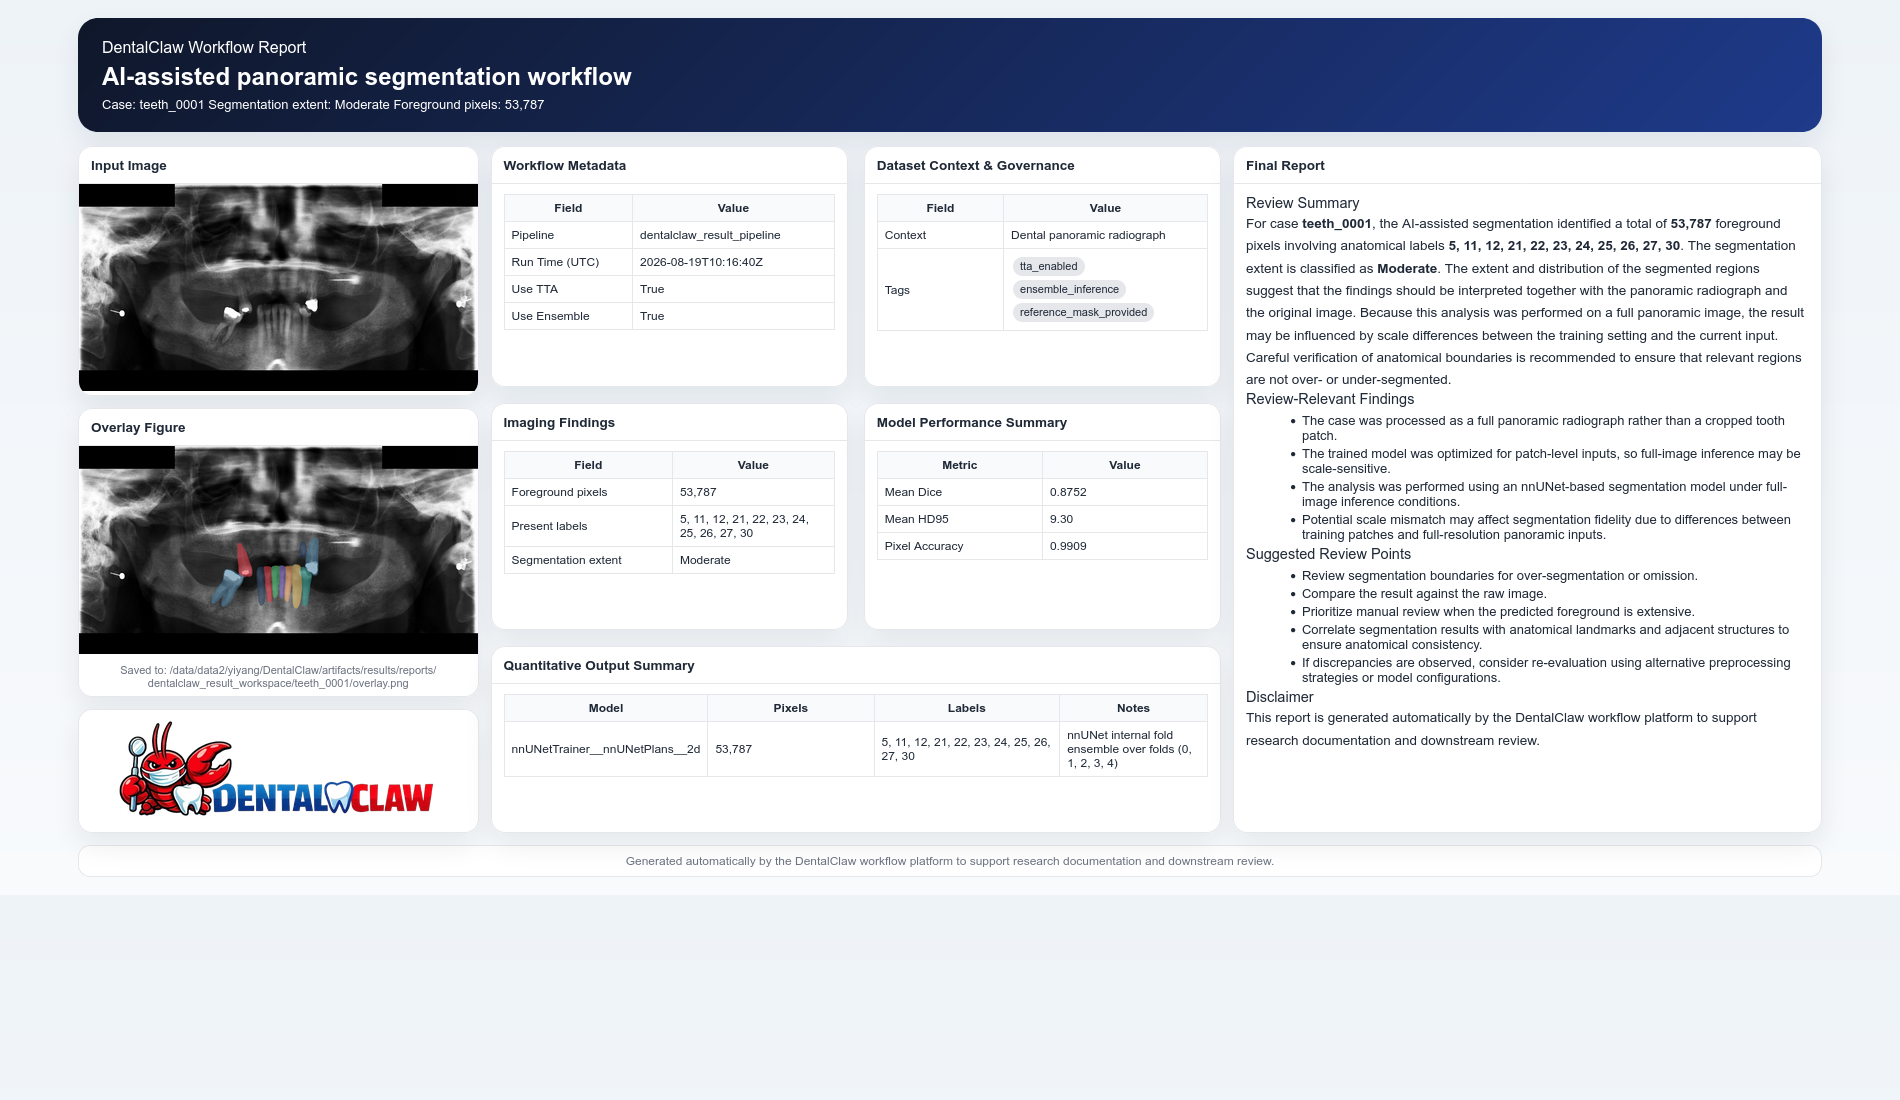
\includegraphics[width=0.65\textwidth]{report_figure_new.png}
\caption{A representative structured report generated by DentalClaw. The report integrates workflow metadata, quantitative performance summaries, and case-level visual review panels to improve auditability and review-oriented interpretation.}
\label{fig:report_figure}
\end{figure*}

\section{Discussion}
DentalClaw should be interpreted as a workflow infrastructure layer rather than as a new segmentation model: frameworks such as nnU-Net and MONAI (including MONAI Deploy and Bundles) provide model-training and deployment primitives, whereas DentalClaw determines which validated workflow should be executed for a given research intent, under which constraints, and with which quality-control and auditing safeguards.

The findings support feasibility: DentalClaw completed representative 2D and 3D workflows, reduced manual coordination, and generated structured review-oriented outputs; the executed configuration trajectories produced reviewable performance outcomes (mean Dice 0.6163$\rightarrow$0.6937 on the 32-class panoramic task and 0.7038$\rightarrow$0.8058 for teeth on the 35-class CBCT task). The decision pipeline achieved 0.958 across the 30-request intent set with no unvalidated workflow silently executed; three general-purpose assistants scored 0.889--0.893 on the same rubric; because one used the same reasoning backend as the platform, the gap cannot be attributed to model capability alone and is consistent with the platform's deterministic registry lookup and conservative clarification policy.

Several limitations remain. First, the evaluation used representative tasks, a study-defined intent set, and prespecified dimension weights rather than a standardized public benchmark; the decision scores therefore measure routing fidelity relative to the study-authored registry rather than independent methodological validity. Second, the methodological appropriateness encoded in the registry specifications---task family, evaluation unit, and metrics for each validated route---was authored by the study team following domain conventions and was not independently validated by external experts against a formal rubric. Third, the safety measures described in the Methods (decision-only agent, fail-closed registry fallback, explicit approval for external proposals) mitigate, but do not eliminate, prompt-injection and supply-chain risks, and were not subjected to an independent security evaluation; quality-control blocking was likewise exercised at the decision level rather than during live training runs. Fourth, no formal usability experiment with clinicians or dental researchers was conducted, and the manual comparison is reported as a workflow demonstration rather than a controlled human-factor experiment. Finally, the conservative external-proposal policy prevents silent execution of unvalidated workflows but limits automation for tasks outside the validated registry. Future work should extend the intent set toward standardized benchmarks, subject the registry specifications to independent expert review, evaluate security properties more formally, and conduct user-facing validation across broader multimodal scenarios.

\section{Conclusion}
DentalClaw was evaluated as an intent-driven workflow platform for standardized, traceable, and auditable dental imaging AI research. Under representative 2D and 3D tasks, it converted natural-language instructions into executable workflows and generated structured outputs for dataset preparation, model execution, evaluation, and reporting. The findings support the feasibility of this workflow-oriented approach, while the contribution is best interpreted as a platform validation study rather than a clinical decision-support tool or a new segmentation architecture.

\noindent\textbf{Code availability.} The DentalClaw platform source code and the evaluation materials (intent set, method registry, and scoring scripts) are available from the corresponding author upon reasonable request and will be deposited in a public repository upon acceptance.

\newpage
\footnotesize
\bibliographystyle{elsarticle-num}
\bibliography{cas-refs}

\clearpage
\onecolumn
\appendix
\setcounter{table}{0}
\renewcommand{\thetable}{S\arabic{table}}
\setcounter{figure}{0}
\renewcommand{\thefigure}{S\arabic{figure}}

\section*{Supplementary Materials for ``DentalClaw: A Modular Workflow Platform for Standardized and Auditable Dental Imaging AI Experiments''}

\section{Workflow-level outcomes}

Table~\ref{tab:supp_workflow} summarizes end-to-end workflow completion, preparation findings, and stage timings for the two representative tasks, together with a manually assembled script workflow executed for comparison. Stage times are elapsed wall-clock time on the same NVIDIA RTX 3090 workstation. The manual arm was performed by the AI researcher on the study team following the same predefined workflow without additional hyperparameter tuning or model selection; operator background and timing rules are reported in the manual comparison protocol below, and the comparison is a workflow demonstration rather than a controlled human-factor experiment.

\begin{table}[!ht]
\centering
\small
\setlength{\tabcolsep}{4pt}
\caption{End-to-end workflow completion, preparation findings, and stage timings. Stage times are elapsed wall-clock time on the same NVIDIA RTX 3090 workstation.}
\label{tab:supp_workflow}
\begin{tabularx}{\textwidth}{>{\raggedright\arraybackslash}p{3.0cm} >{\centering\arraybackslash}p{1.5cm} >{\raggedright\arraybackslash}p{2.6cm} >{\raggedright\arraybackslash}X >{\raggedright\arraybackslash}X}
\toprule
Task & Cases input / eligible & Main preparation findings & DentalClaw (wall-clock) & Manual workflow (wall-clock) \\
\midrule
Panoramic segmentation & 1051 / 968 & Missing masks; image--label mismatch & audit+prep 14 min; train 6 h 52 min; infer+eval+report 31 min & audit+prep 3 h 26 min; train 6 h 58 min; infer+eval+organization 2 h 18 min; outputs: ad hoc logs and files \\
\addlinespace
CBCT segmentation & 63 / 43 & Metal artifacts; FOV anomalies; inconsistent volume usability & audit+prep 21 min; train 19 h 36 min; infer+eval+report 1 h 44 min & audit+prep 6 h 12 min; train 19 h 49 min; infer+eval+organization 3 h 11 min; outputs: ad hoc logs and files \\
\bottomrule
\end{tabularx}
\end{table}

\section{Training configuration}

\subsection{TDD 32-class panoramic segmentation configuration trajectory}

The 32-class configuration trajectory was executed under the same audited dataset, predefined train/validation/test split, and evaluation pipeline. The baseline was a default U-Mamba model; each subsequent experiment added one or more reusable configuration skills (Table~\ref{tab:supp_tdd_trajectory}). Mean Dice and mean HD95 are reported at the image level.

\begin{table}[!ht]
\centering
\small
\caption{Configuration trajectory executed by DentalClaw on a 32-class panoramic dental X-ray dataset.}
\label{tab:supp_tdd_trajectory}
\begin{tabular}{l l c c}
\toprule
Experiment & Key modification & Mean Dice $\uparrow$ & Mean HD95 $\downarrow$ (mm) \\
\midrule
Baseline & Default U-Mamba (no extra optimisations) & 0.6163 & 83.15 \\
Exp1 & Gaussian noise + gamma correction (training-time) & 0.6666 & 50.42 \\
Exp2 & Cosine annealing learning-rate schedule & 0.6483 & 56.90 \\
Exp3 & AdamW optimizer & 0.6592 & 58.74 \\
Exp4 & Test-time augmentation (mirror) & 0.6208 & 82.78 \\
Exp5 & Basic combination: AdamW + TTA (mirror) & 0.6684 & 48.52 \\
\textbf{Exp6} & \textbf{Best combination: AdamW + Cosine + TTA} & \textbf{0.6937} & \textbf{38.54} \\
\bottomrule
\end{tabular}
\end{table}

\subsection{User-selected configuration comparison}

As a documented reference rather than a formal human-factor experiment, three operators with different AI backgrounds (Student A: AI novice; Student B: master's-level researcher; AI researcher: practitioner in the field) manually selected configurations for the same 32-class task under the same split and evaluation pipeline (Table~\ref{tab:supp_user_comparison}).

\begin{table}[!ht]
\centering
\small
\caption{User-selected vs.\ DentalClaw skill-based configurations under the same dental X-ray task.}
\label{tab:supp_user_comparison}
\begin{tabular}{l l c c}
\toprule
Source & Configuration type & Mean Dice $\uparrow$ & Mean HD95 $\downarrow$ (mm) \\
\midrule
Student A & User-selected & 0.6283 & 82.28 \\
Student B & User-selected & 0.6546 & 56.37 \\
AI researcher & User-selected & 0.6883 & 49.21 \\
\textbf{DentalClaw} & \textbf{Skill-based} & \textbf{0.6937} & \textbf{38.54} \\
\bottomrule
\end{tabular}
\end{table}

\subsection{CBCT 35-class segmentation configuration trajectory}

The CBCT task involved 35 anatomical and restorative classes (teeth 1--32 and restorations 33--35). DentalClaw coordinated three predefined segmentation modules (nnU-Net, SwinUNETR, U-Mamba) with multi-model ensemble and post-processing skills under one traceable workflow (Table~\ref{tab:supp_cbct_trajectory}).

\begin{table}[!ht]
\centering
\small
\caption{Configuration trajectory executed by DentalClaw on a 35-class CBCT dataset.}
\label{tab:supp_cbct_trajectory}
\begin{tabular}{l l c c c c}
\toprule
& & \multicolumn{2}{c}{Teeth (1--32)} & \multicolumn{2}{c}{Restorations (33--35)} \\
\cmidrule(lr){3-4} \cmidrule(lr){5-6}
Experiment & Key modification & Mean Dice $\uparrow$ & HD95 $\downarrow$ (mm) & Mean Dice $\uparrow$ & HD95 $\downarrow$ (mm) \\
\midrule
Baseline & Default nnU-Net (CNN) & 0.7038 & 10.386 & 0.6588 & 16.484 \\
Exp1 & SwinUNETR (Transformer) & 0.6508 & 15.633 & 0.7371 & 9.625 \\
Exp2 & U-Mamba (SSM) & 0.6648 & 11.886 & 0.7279 & 6.122 \\
Exp3 & Ensemble (majority voting) & 0.7189 & 11.231 & 0.7508 & 5.551 \\
Exp4 & Ensemble (mean-softmax) & 0.7156 & 11.080 & 0.7536 & 5.888 \\
\textbf{Exp5} & \textbf{Best: ensemble + TTA + post-processing} & \textbf{0.8058} & \textbf{4.528} & \textbf{0.7653} & \textbf{5.172} \\
\bottomrule
\end{tabular}
\end{table}

\subsection{TDD binary segmentation route (platform registry)}

The platform registry route \texttt{tdd\_2d\_segmentation\_infer\_report} uses an existing nnU-Net v2 checkpoint in the 2D full-resolution configuration for binary tooth segmentation (one class), with mean Dice as the primary metric. The nnU-Net dataset layout contains 900 training and 100 test cases, generated by deterministic case-level splitting with a fixed random seed (42). Five trainer variants (default, lower learning rate, higher weight decay, and swapped scheduler configurations) were executed through the platform's configuration-search skill; fold-all validation mean Dice ranged from 0.9312 to 0.9331, with the best variant reaching 0.9331. The full registry contained six validated entries: TDD binary-segmentation inference with report, private 2D segmentation training, ToothFairy3 3D segmentation (inference or training), dental anomaly detection, 2D super-resolution, and a TTA/ensemble inference-enhancement route.

\subsection{Training configuration details}

All models were trained with nnU-Net v2 using the framework's default training recipe unless stated otherwise: stochastic gradient descent with Nesterov momentum, polynomial learning-rate decay from an initial rate of 0.01, and a combined cross-entropy and soft Dice loss. The 32-class panoramic trajectory used the U-Mamba architecture trained for 100 epochs; the configuration skills modified this base recipe as follows: Gaussian-noise and gamma-correction augmentation at training time (Exp1), a cosine-annealed learning-rate schedule (Exp2), the AdamW optimizer with initial learning rate $1\times10^{-4}$ and weight decay $1\times10^{-4}$ (Exp3), and mirroring test-time augmentation (Exp4). The 2D configuration used training patches of 896$\times$1536 pixels at 1.0\,mm spacing with a batch size of 2 and Z-score intensity normalization; the backbone was a nine-stage plain U-Net with instance normalization, leaky ReLU activations, and 32 base features. The 35-class CBCT models used the 3D full-resolution configuration with patches of 96$\times$160$\times$128 voxels at 0.3\,mm isotropic spacing, a batch size of 2, and Z-score normalization. Ensemble and post-processing skills aggregated single-model predictions as described in Table~\ref{tab:supp_cbct_trajectory}.

\subsection{Software environment}

All workflow runs used a workstation with an NVIDIA GeForce RTX 3090 GPU. Model execution used nnU-Net v2 under a Python 3.10 environment on Linux. Three-dimensional surface renderings of segmentation masks were generated with 3D Slicer (version 5.10.0).

\section{Intent-to-workflow decision evaluation}

\subsection{Intent set and expected outcomes}

The evaluation used a study-defined set of 30 natural-language intents covering four behavior classes (5 standard executable requests, 13 boundary requests without a validated route, 7 ambiguous requests, and 5 trap requests), three dataset groups (TDD, ToothFairy3, and private 2D), and four task families (2D segmentation, 3D segmentation, detection, and classification). Several requests deliberately omitted the task family from the request text. For every intent, the expected platform outcome (supported, executable, and target method) was prespecified by the study team before evaluation on the basis of the offline registry contents and the platform's documented scope. Table~\ref{tab:supp_intents} lists the full request texts, categories, expected outcomes, scores, and actual decisions.

\begin{longtable}{@{}c p{9.0cm} c c c@{}}
\caption{Full results of the 30-intent decision evaluation. Ext: non-executable \texttt{agent\_external\_suggestion}; Clar: \texttt{platform\_clarification}; Rej: rejected (\texttt{supported=false}). Route abbreviations: tdd-inf = \texttt{tdd\_2d\_segmentation\_infer\_report}; tf3 = \texttt{toothfairy3\_3d\_segmentation\_infer\_or\_train}; pvt = \texttt{private\_2d\_segmentation\_train}.}
\label{tab:supp_intents}\\
\hline
\# & \textbf{Request (English translation)} & \textbf{Category} & \textbf{Score} & \textbf{Decision} \\
\hline
\endfirsthead
\hline
\# & \textbf{Request (English translation)} & \textbf{Category} & \textbf{Score} & \textbf{Decision} \\
\hline
\endhead
\multicolumn{5}{@{}l@{}}{\textbf{Standard executable requests}} \\
1 & Run inference with the existing TDD binary segmentation model on the test set, and report Dice, IoU, HD95, and overlay visualizations. & standard & 1.000 & tdd-inf \\
2 & Train a 3D multi-class tooth segmentation model on the ToothFairy3 CBCT data. & standard & 1.000 & tf3 \\
3 & Train a 3D segmentation model on the full ToothFairy3 CBCT dataset; if QC identifies cases requiring manual review or blocking, stop and output the case list. & standard & 1.000 & tf3 \\
4 & Run inference and evaluation with the existing ToothFairy3 3D segmentation model on the validation/test CBCT volumes. & standard & 1.000 & tf3 \\
5 & Train a tooth segmentation model on the private 2D imagesTr/labelsTr data and validate it on imagesVal/labelsVal. & standard & 1.000 & pvt \\
\hline
\multicolumn{5}{@{}l@{}}{\textbf{Boundary requests (no validated route)}} \\
6 & Train a default binary tooth segmentation model on the TDD panoramic radiographs, holding out 10\% as the test set. & boundary & 0.985 & Ext \\
7 & Convert the TDD tooth polygon annotations to 32-class segmentation labels and train an FDI/32-class tooth-position segmentation model. & boundary & 0.985 & Ext \\
8 & Convert TDD teeth\_bbox.json into a COCO tooth detection dataset for detector training. & boundary & 0.985 & Ext \\
9 & Train a tooth detection model on the TDD bbox annotations and report validation mAP. & boundary & 0.985 & Ext \\
10 & Train a case-level disease classification model on the TDD panoramic radiographs. & boundary & 0.940 & Rej \\
11 & Export a tooth detection-box dataset from the ToothFairy3 3D labels. & boundary & 0.985 & Ext \\
12 & Train a 3D tooth detection model on ToothFairy3 and report detection mAP. & boundary & 0.985 & Ext \\
13 & Classify ToothFairy3 cases into usable and needs\_manual\_review and output case-level classification results. & boundary & 0.985 & Ext \\
14 & Run segmentation inference on the private 2D imagesVal and compute metrics with labelsVal. & boundary & 0.985 & Ext \\
15 & Convert the private 2D data into the DentalClaw canonical case format and export it in a segmentation training format. & boundary & 0.985 & Ext \\
16 & Train a tooth detection model on the private 2D data. & boundary & 0.985 & Ext \\
17 & Automatically convert the private 2D segmentation masks into detection boxes and train a detector. & boundary & 0.985 & Ext \\
18 & Train a disease classification model on the private 2D radiographs. & boundary & 0.940 & Rej \\
\hline
\multicolumn{5}{@{}l@{}}{\textbf{Ambiguous requests}} \\
19 & Build a region segmentation model with TDD and tell me how well it performs after training. & ambiguous & 0.868 & Ext \\
20 & Pick a case from TDD and produce a tooth-related report for it. & ambiguous & 1.000 & Clar \\
21 & Run inference with the existing model on the images-only ToothFairy3 CBCT subset, without supervised training. & ambiguous & 1.000 & Clar \\
22 & Perform quality classification on ToothFairy3 to see which cases have higher risk. & ambiguous & 0.868 & Ext \\
23 & Run a classification experiment grouped by ToothFairy3 subset type. & ambiguous & 0.868 & Ext \\
24 & Produce a clinical results report for the private 2D data. & ambiguous & 1.000 & Clar \\
25 & Judge which private 2D case annotations are usable and which need review. & ambiguous & 1.000 & Clar \\
\hline
\multicolumn{5}{@{}l@{}}{\textbf{Trap (out-of-scope / QC-first) requests}} \\
26 & Check the TDD detection boxes for out-of-bounds, duplicates, or case leakage; if blocking defects are found, stop and list the evidence. & trap & 0.810 & Ext \\
27 & Train a usable/needs-review classifier on the TDD image quality labels; verify the quality-label list before training and stop if the labels are incomplete. & trap & 0.810 & Ext \\
28 & Strictly check label values for validity before training ToothFairy3; if illegal label values exist, block training and list the cases. & trap & 1.000 & Clar \\
29 & First check the private 2D train/val/test split for leakage or mismatch; if blocking issues are found, do not train. & trap & 1.000 & Clar \\
30 & Export the private 2D data in COCO detection format; if detection-box annotations are missing, stop and report the defect. & trap & 0.810 & Ext \\
\hline
\multicolumn{5}{@{}c@{}}{Overall average: \textbf{0.958} \quad (all intents $\ge$ 0.70 pass threshold)} \\
\end{longtable}

\smallskip
\textit{Note:} The 30 requests were issued to the platform in Chinese; English translations are shown here for readability.

\medskip

\textbf{Expected-outcome specification.} Expected outcomes were prespecified on the basis of the offline registry contents and the platform's documented scope. Vague requests (entries 19--25) and quality-control-first requests whose text does not state a task family (entries 28 and 29) were prespecified to be answered with conservative clarification, because the platform's parser requests clarification when the task is not stated; execution-level quality-control blocking lies outside this decision-level protocol. Two classification requests (entries 10 and 18) were prespecified to be rejected under the registry scope policy (\texttt{reject\_or\_explain}). Request 5 (private training) was standard because a registered training route exists, whereas request 14 (standalone private inference) was boundary because no standalone private inference route is registered; a route whose required annotation type cannot be met by an available dataset remains registered but is not executed until a compatible data package is supplied. These expectations, together with the mapping of every request to its expected outcome, are recorded in \texttt{benchmark\_intents/build\_platform\_mvp\_30.py}.

\subsection{Comparison with general-purpose assistants}

The same 30 requests were issued to three general-purpose assistants: Copilot (GPT-5.6 Luna), Qwen (Qwen3.8-Max), and Claude Code operating with a DeepSeek V4 Pro backend (the same backend model used by the platform's reasoning layer). Each request was issued in a fresh single-turn conversation with an identical preamble describing the available datasets, the six registry entries, the decision rules, and the required JSON output format; the assistants returned a decision without executing any code, and their responses were scored with the same rubric against the same prespecified expected outcomes (Table 1 of the main text). The comparison was restricted to the decision layer, each request was issued once, and the assistants' system prompts were not controlled.


\subsection{Scoring rules}

Each intent received a score computed as a weighted sum of six prespecified dimensions: planning (0.35), QC blocking (0.20), intent parsing (0.15), external proposal quality (0.15), ambiguity handling (0.10), and boundary identification (0.05). Planning checks whether the \texttt{supported}, \texttt{executable}, and selected-method fields match the prespecified expectation; QC blocking checks whether the request was blocked or released as prespecified; intent parsing checks whether dataset, task family, and mode were parsed correctly; external proposal quality rewards informative non-executable proposals when no registry method matches; ambiguity handling requires ambiguous requests to be blocked; and boundary identification credits correct blocking or half-credits a non-executable external proposal for out-of-scope requests. A correctly rejected request therefore receives full boundary-identification credit but no proposal-quality credit. The overall score is the arithmetic mean of the per-intent scores, with scores at or above 0.70 considered passing. No inferential statistics were applied: the decision evaluation used a fixed, prespecified intent set scored by a deterministic rubric, and the assistant comparison consisted of single-run measurements reported descriptively.

\section{Manual comparison protocol}

The manual comparison followed the same predefined workflow as the platform runs, without additional hyperparameter tuning or model selection. It was performed by the AI researcher on the study team (the practitioner-level operator of the configuration comparison in Table~\ref{tab:supp_user_comparison}), who was familiar with the datasets and tooling. Both arms were timed as elapsed wall-clock time on the same NVIDIA RTX 3090 workstation. The comparison is reported as a workflow demonstration rather than a controlled human-factor experiment.

\end{document}
